\setcounter{ExampleCounter}{1}
\begin{center}

\includegraphics[width=0.8\textwidth]{Census2020Logo}
\end{center}
Every 10 years, the U.S. Census Bureau undertakes the enormous task of gathering all kinds of data on people residing in the country.  This is incredibly difficult, but equally important, because everything from representation in Congress to federal funding depends on having accurate counts.

It's not hard to see why this process is so complicated.  Not only are there hundreds of millions of people in the country, but many live in rural areas, others are transient or homeless, and many may be suspicious of someone showing up at their door with a clipboard, asking questions.  Because of this, and because it is crucial to count everyone, not just those who are easy to count, the Census Bureau devotes a tremendous amount of time, energy, and money to designing their procedure as carefully as possible.

\subsection{Sampling}
Now think of a different example: a presidential election.  The election occurs on a specific day, and you can think of the election as a massive survey with the question, ``Who do you want to be President?''

However, before the election occurs, we generally like to have an idea of how the vote will turn out.  How can we predict it?  Can we go around and ask every voter how they plan to vote, and then repeat this every so often (because people may change their minds)?  Clearly, that's impractical, so we turn to the statistician's secret weapon: \textbf{sampling}.

To understand why sampling works, think about cooking a pot of soup.  Throughout the process, a good cook will frequently take a small spoonful from the simmering pot and taste it.  The cook doesn't need to eat the entire potful to get a sense of how it's doing; even though there are many ingredients in the pot, if it is well-stirred, the small spoonful will taste the same as the entire pot, more or less.

This is exactly what happens when a statistician selects a sample to make a prediction.  Rather than surveying every voter, if we carefully choose a relatively small group of voters and ask them the question, ``Who do you plan to vote for?'' we can assume that the mixture of answers will be relatively close to the mixture in the full population of voters.

\begin{formula}{Population and Sample}
\paragraph{Population:} the full group that we're interested in understanding.\\
\emph{Example: everyone who will vote on Election Day}

\paragraph{Sample:} a small group chosen from the population that we use to estimate the response of the full group.\\
\emph{Example: a few voters chosen to take a poll}
\end{formula}

Because it is generally not possible or feasible to study the entire population, nearly every statistical study involves taking a sample, and using that sample to predict what the population looks like.

\begin{example}[https://www.youtube.com/watch?v=-AK3lL3YKOA&list=PLfmpjsIzhzttL_Uec2nCbDRcAcUF7NKG8&index=1]{Pet Ownership}
A sample of 2,000 households in the U.S. was selected and asked if they currently own at least one pet. The results show that 69\% of households do own at least one pet.
Identify the sample and population in this situation.

\sol
The sample is the 2,000 households and the population is all households in the U.S. Notice that even though the population is not explicitly stated, we can infer it from carefully reading the sentence. 
\end{example}

\begin{try}[http://hartleymath.com/versatilemath/tryit/\#/statistics--sample-and-population]
A researcher wants to know how citizens of Frederick City felt about a voter initiative. To study this, she goes to the Francis Scott Key Mall in the city, randomly selects 500 shoppers and asks them their opinion. Sixty percent indicate they are supportive of the initiative. What is the sample and population?
\end{try}

\subsection{The Importance of Randomness}
You may have spotted a potential pitfall already: what guarantee do you have that your sample will be a good measure of the population.  To use the term that statisticians do, how do you know that you have a \emph{representative sample}?

\begin{center}
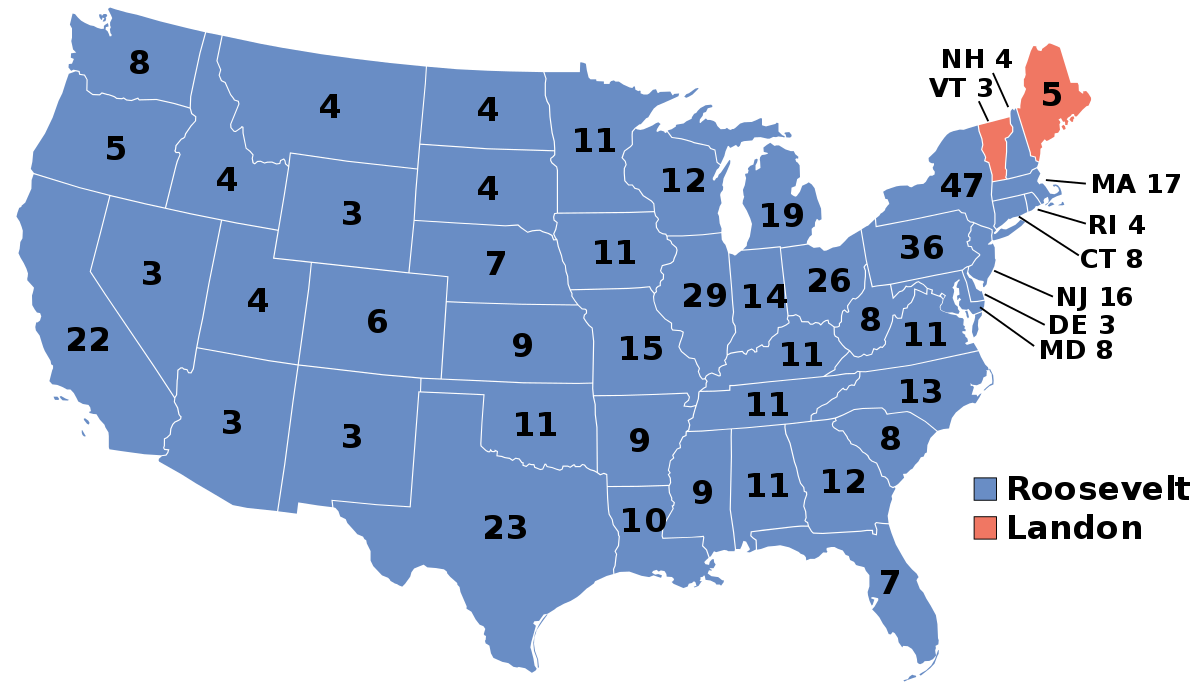
\includegraphics[width=0.6\textwidth]{1936ElectoralCollege}
\end{center}

To see how this can go wrong, let's go back to 1936.  The nation was in the midst of the Great Depression, and the incumbent Democrat, Franklin Roosevelt, was challenged by the Republican governor of Kansas, Alf Landon.  President Roosevelt was working to enact portions of his New Deal, and while Governor Landon agreed with parts of the New Deal, he criticized it for waste and inefficiency.

As you can see on the map above, Roosevelt was reelected in the most lopsided victory in American history (in terms of electoral votes).  He even carried Landon's home state of Kansas, and of the states he won, few were close; only four of those states had a margin of victory of less than 10 percentage points.

So in the months leading up to the most one-sided election result ever, certainly it was clear that Roosevelt would win, right?  Not so fast.  A magazine called the \emph{Literary Digest} boasted that it had correctly predicted the results of the previous five elections.  Their approach was to select a \emph{huge} sample of millions of potential voters.  The \emph{Digest} sent out 10 million questionnaires and received over 2 million responses.  What did their data say?  It predicted that Landon would cruise to an easy victory.\\

How could they have gotten it so wrong?  Their fundamental error was in thinking that a \emph{larger} sample would be more reliable, rather than a more carefully chosen \emph{representative} sample.  This would be like a cook who decided that they needed to eat an entire bowl of soup to know how it tastes, rather than carefully stirring before selecting a small spoonful.

Let's take a closer look at the \emph{Digest}'s method.  They started by surveying their own readers, and then they turned to automobile registrations and telephone directories to gather names and addresses to which to send their questionnaire.  That was their first error.

Remember how they sent out 10 million surveys and received 2 million responses?  This is a red flag, because their survey was a \emph{voluntary response} survey, in which people had to take initiative to respond.  That was their second error.

First of all, their flawed sampling method skewed the sample toward more wealthy people.  Remember that this took place in the midst of the Great Depression, so people who had the disposable income for a magazine subscription, or owned a car or telephone, were likely to be wealthier than the average voter.  These wealthier voters had less stake in the policies of the New Deal, and since they were less likely to take advantage of its benefits, they were more likely to agree with Governor Landon that the New Deal was wasteful and inefficient.

Second, since people had to take an active step (filling out the questionnaire and mailing it in), responses were more likely to come from people who felt strongly about the question, and this tends to attract people who are unhappy with the status quo (remember that Roosevelt was the incumbent).  People who were mostly content with the direction of the country, who would vote to re-elect Roosevelt, were less inclined to respond.  This is a major problem with voluntary response surveys in general, and the main reason that they are generally considered unreliable.

Largely due to the very public failure of their polling system, the \emph{Literary Digest} folded in less than two years.  The same election, though, saw the debut of the well-known Gallup poll, when a pollster named George Gallup used a much smaller, carefully chosen sample to correctly predict the results.\\

What's the lesson?  When sampling, \textbf{a representative sample is better than a large sample}.  Remember the metaphor of the pot of soup; larger samples might improve the results, but not by as much as carefully stirring the pot first.

\begin{example}[https://www.youtube.com/watch?v=f-RqidmHOjc&list=PLfmpjsIzhzttL_Uec2nCbDRcAcUF7NKG8&index=2]{Representative Samples}
Decide whether each of the following sampling methods is likely to produce a representative sample.

\begin{enumerate}[(a)]
\item To find the average annual income of all adults in the United States, sample representatives in the US Congress.
\item To find out the most popular cereal among children under the age of 10, stand outside a large supermarket one day and poll every twentieth child under the age of 10 who enters the supermarket.
\end{enumerate}

\sol
\begin{enumerate}[(a)]
\item This is probably \textbf{not representative}, if for no other reason than that the salary of congresspeople is fixed by law at a single value.  It happens to be much higher than the average salary in the U.S., but this is partly by design, in order to reduce the incentive to accept bribes.

\item This seems likely to be \textbf{representative}; while there could be regional differences, for instance, there are no obvious biases.
\end{enumerate}
\end{example}

Okay, so if we want a good, representative sample, how do we do this?  How do we make sure that our sample looks like the population (that, for instance, the racial and ethnic proportions match)?  This is a hard question; in fact, it is so hard that we don't directly tackle it.\footnote{At times, pollsters \emph{do} adjust their samples to reflect some demographic trends.}  Instead, we rely on \textbf{randomness}.

\begin{proc}{Representative Samples}
Random selection leads to representative samples.
\end{proc}

Say you have a question about the behavior of college students, like how much they spend on textbooks in a typical semester.  There are all sorts of variations that you may or may not think of; for instance, it may depend on what year they are in, since senior-level textbooks may be more expensive.  It may depend on what major they are in, what college or university they attend, and a hundred other factors that may not even occur to you.  You could try to build an exhaustive list of all of these factors, and then decide to get equal numbers of students in each year.  Maybe then you figure out the proportions of students in each major and try to match those proportions in your sample.  Is it starting to sound like a really thorny problem?

Instead, if you can find a good way to \emph{randomly} select college students, the problem will take care of itself.  If students are divided evenly in freshmen, sophomores, juniors, and seniors, and you truly select people randomly, probability suggests that you will select \emph{approximately} a quarter of your sample from each group.
\pagebreak

\begin{proc}{Random Samples}
The key to a random sample is that \textbf{each member of the population is equally likely to be selected}.
\end{proc}

\paragraph{Examples of Random Samples}
\begin{itemize}
\item If the population is students in a particular classroom, number the students in the classroom from 1 to $n$ and use a random number generator to select numbers between 1 and $n$.
\item If the population is FCC students, list their FCC email accounts and number them, then pick random numbers between 1 and $n$, where $n$ is the number of students.
\end{itemize}

\paragraph{Examples of Biased Samples}
\begin{itemize}
\item \marginnote{Not every resident of the county has a phone, let alone a phone listed in the phone book}If the population is residents of Frederick County, number the entries in the phone book and use a random number generator to select a sample.
\item If the population is American citizens, go to the entrance of Yankee Stadium and poll everyone entering.
\item If the population is FCC students, poll the students in one class.
\end{itemize}

If you're ever unclear on whether or not a sampling method is random, simply ask whether or not every member of the population has an equal chance of being selected.

\subsubsection*{Picking Random Numbers with a Graphing Calculator}
Your graphing calculator can select random numbers.  To access this menu, press the \calcbutton{MATH} button and use the left and right arrows to navigate to the PRB (probability) tab.
\begin{center}
\begin{tabular}{c | c}
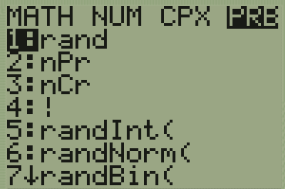
\includegraphics[height=0.9in]{RandMenu}
& 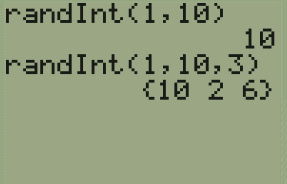
\includegraphics[height=0.9in]{randInt}\\
\parbox{0.45\textwidth}{Selecting \texttt{rand} will select a ``random'' (technically pseudo-random, but close enough for us) number between 0 and 1.  Selecting \texttt{randInt(} will allow you to choose a random integer between a given lower and upper bound, or several of those.}
& \parbox{0.45\textwidth}{To select a single random integer, enter \texttt{randInt(}lower bound\texttt{,}upper bound\texttt{)}, with whatever numbers you want for the lower and upper bounds.  To select $n$ random integers, enter \texttt{randInt(}lower bound\texttt{,}upper bound\texttt{,}$n$\texttt{)}}
\end{tabular}
\end{center}

\begin{example}[https://www.youtube.com/watch?v=mm1iQfMgNHE&list=PLfmpjsIzhzttL_Uec2nCbDRcAcUF7NKG8&index=3]{Cartwheels}
A coach is interested in how many cartwheels the average college freshman can do at his university. Eight volunteers from the freshman class step forward. After observing their
performance, the coach concludes that college freshmen can do an average of 16 cartwheels in a row without stopping. Is this sample random and representative?

\sol
The population is the class of all freshmen at the coach's university. The sample is composed of all freshmen so that is good. However, the sample is poorly chosen because volunteers are more likely to be able to do cartwheels than the average freshman: people who cannot do cartwheels probably did not volunteer! Hence, this sample is not random, and thus unlikely to be representative.
\end{example}

\begin{try}
A substitute teacher wants to know how students in the class did on their last test. The teacher asks the 10 students sitting in the front row to state their latest test score. He concludes from their responses that the class did extremely well. What is the sample and population? Is the sample random and representative? Why or why not?
\end{try}

\subsection{Sampling Methods}

Naturally, this brings up another question: how do we pick a random sample?  There are many ways to do this; let's look at a few.

\begin{formula}{Simple Random Sampling}
Number every member of the population and use a random number generator (like a calculator) to pick as many members as you need for the sample. 
\end{formula}

Simple random sampling is the most common method; most studies default to this one unless there's a good reason to use a more exotic approach.  The hardest part is often acquiring as thorough a list of the population as possible.

\begin{formula}{Convenience Sampling}
Pick members of the population that are easy to pick. 
\end{formula}

Convenience sampling is generally not as reliable as other methods, but it is the easiest.  There are cases, though, where the benefits outweigh the costs.  For instance, say you were the quality assurance officer at a facility that manufactured something heavy like cinder blocks.  If a full pallet is delivered, and you need to select a few blocks to test for strength, a simple random sample would require digging through the full stack and moving a lot of the blocks.  Instead, you could assume that this pallet all comes from the same batch, and so testing one of the blocks on the top layer will give you a representative idea of the batch quality.  It can be dangerous to make assumptions, but those with specialized knowledge can sometimes do so.

\begin{formula}{Systematic Sampling}
Randomly pick a starting point and select every $n$th member.
\end{formula}

With systematic sampling, the randomness all comes from the random starting point, so that part of the process is crucial; you can't start from the beginning of the list and select every third person and call that systematic sampling.

\begin{formula}{Stratified Sampling}
Divide the population into categories (for instance, divide college students into freshmen, sophomores, juniors, and seniors), then randomly select an equal number from each category.
\end{formula}

\begin{formula}{Cluster Sampling}
Like stratified sampling, divide the population into groups, but this time, select one or more \emph{entire} groups, rather than a few from each group.
\end{formula}

It's easy to confuse stratified and cluster sampling, because they sound similar.

\begin{center}
\begin{tabular}{c c}
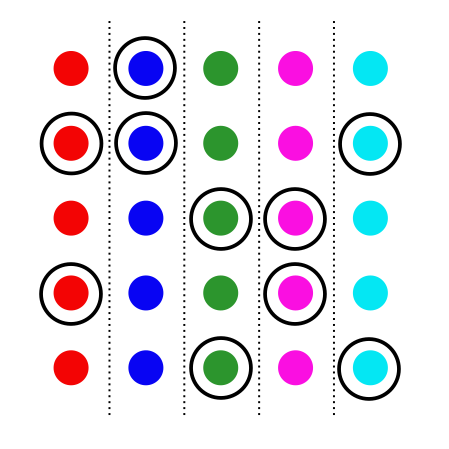
\includegraphics[height=1.2in]{StratifiedSampling}
& 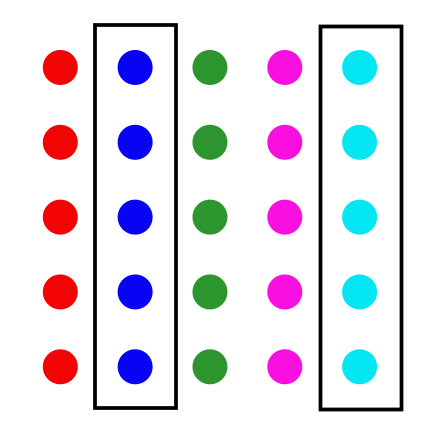
\includegraphics[height=1.2in]{ClusterSampling}\\
{\small Stratified sampling} & {\small Cluster sampling}
\end{tabular}
\end{center}

Stratified sampling means picking a few from \emph{each} cluster; cluster sampling means selecting a few \emph{entire} clusters.

For instance, suppose you're canvassing a neighborhood to poll residents about a new local ordinance, and say this neighborhood consists of 10 apartment building, with 12 apartments in each building.  If you decided to use stratified sampling, you could enter each building and use a random number generator to pick 2 apartments; this would give you a random sample of 20 homes.  On the other hand, if you used cluster sampling, you could randomly select two buildings and survey every apartment in those buildings, for a total of 24 responses.  In this case, if there's no need to get a response from each building, cluster sampling would be more convenient, since you wouldn't need to travel as far.

\begin{example}[https://www.youtube.com/watch?v=AkdmTILWkgk&list=PLfmpjsIzhzttL_Uec2nCbDRcAcUF7NKG8&index=4]{Sampling Methods}
Determine the type of sampling used in each of the following scenarios.

\begin{enumerate}[(a)]
\item A soccer coach selects six players from a group of boys aged eight to ten, seven players from a group of boys aged 11 to 12, and three players from a group of boys aged 13 to 14 to form a recreational soccer team.

\sol
This is \textbf{stratified sampling}, since the group is divided into categories, and a few are taken from each category.

\solline
\item A pollster interviews all human resource personnel in five different high tech companies.

\sol
This sounds like \textbf{cluster sampling}; the companies are the clusters, and these five companies have been selected in entirety.

\solline
\item A high school educational counselor interviews 50 female teachers and 50 male teachers.

\sol
This is \textbf{stratified sampling}, with teachers categorized by gender.

\solline
\item A medical researcher interviews every third cancer patient from a list of cancer patients at a local hospital.

\sol
The key here is that \emph{every third} patient is selected; that's the sign of \textbf{systematic sampling}.

\solline
\item A high school counselor uses a computer to generate 50 random numbers and then picks students whose names correspond to the numbers.

\sol
There are no categories, and no systematic progression through a list; this is purely random, and indeed is \textbf{simple random sampling}.

\solline
\item A student interviews classmates in his algebra class to determine how many pairs of jeans a student at his school owns, on the average.

\sol
Since this student simply interviews the nearest available students, this represents \textbf{convenience sampling}; there was no attempt at randomness.
\end{enumerate}
\end{example}
\pagebreak

\begin{example}[https://www.youtube.com/watch?v=Ix-PKoZrJks&list=PLfmpjsIzhzttL_Uec2nCbDRcAcUF7NKG8&index=5]{Quiz Score Samples}
% for consistency, use 12345 as the seed
Use the random number generator on your calculator to generate different types of samples from the data below.  Find the average score for each sample and compare the results for each method.\\

This table displays six sets of quiz scores (out of 10 points) for an elementary statistics class.
\begin{center}
\begin{tabular}{l l l l l l}
A & B & C & D & E & F\\
\hline
& & & & & \\
5 & 7 & 10 & 9 & 8 & 3\\
10 & 5 & 9 & 8 & 7 & 6\\
9 & 10 & 8 & 6 & 7 & 9\\
9 & 10 & 10 & 9 & 8 & 9\\
7 & 8 & 9 & 5 & 7 & 4\\
9 & 9 & 9 & 10 & 8 & 7\\
7 & 7 & 10 & 9 & 8 & 8\\
8 & 8 & 9 & 10 & 8 & 8\\
9 & 7 & 8 & 7 & 7 & 8\\
8 & 8 & 10 & 9 & 8 & 7\\
\end{tabular}
\end{center}

Create a sample of 12 scores using each of the following methods.
\begin{enumerate}[(a)]
\item Stratified sampling
\item Cluster sampling
\item Simple random sampling
\item Systematic sampling
\item Convenience sampling
\end{enumerate}

\sol
\begin{enumerate}[(a)]
\item To create a stratified sample, we need to decide what to use as the categories (also called \emph{strata}).  Since the data is separated into 6 categories already (A-F), we can take advantage of this natural division.  To get a sample of 12 scores, we need to select 2 from each category.  We'll show the process for group A, but omit the rest, since it follows the same pattern.\\

Group A: to select two scores from this category, we need to generate two random values between 1 and 10 (since there are 10 scores in the group).  We'll use the \texttt{randInt} function on the calculator.  Remember, to access this, press the \calcbutton{MATH} button and navigate to the \texttt{PRB} menu, then look for the option labeled \texttt{5: randInt(}.  Since we want two values, we'll type in \texttt{randInt(1,10,2)} (the comma button is above the \calcbutton{7} key).
\begin{center}
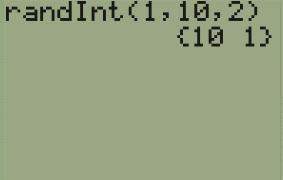
\includegraphics[width=1.6in]{samplingExRandInt}
\end{center}
This means that we have selected the 10th and 1st values in the list; if we scan down the list in the first column, the 10th value is 8 and the 1st value is 5, so the first two values in our sample are 8 and 5.\\

For the other groups, we repeat this process.  If you follow along on your calculator, you may get different results, but the final sample is
\[\boxed{8, 5, 7, 7, 9, 10, 9, 5, 7, 7, 4, 7}\]

We'll cover this in more detail in another section, but you are probably familiar with the average; to calculate it, add up all the values and divide by how many values there are.
\begin{align*}
\textrm{Average score: } &= \dfrac{8+5+7+7+9+10+9+5+7+7+4+7}{12}\\
&= \boxed{7.1}
\end{align*}

\item Since we want a total of 12 scores in our sample, we need to define clusters in such a way that a few of them will total 12 in size.  We could, of course, define the columns to be the clusters, but then if we selected two columns, for instance, we would need to toss out some values.\\

Instead, it will be simpler to define the rows of the table as the clusters; this way, we can randomly select two of them and wind up with 12 values.  Use the calculator as before; this time, we only need to select random values once:
\begin{center}
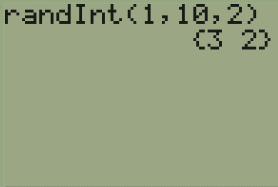
\includegraphics[width=1.6in]{samplingExRandInt2}
\end{center}
We selected the 2nd and 3rd rows, so the sample consists of these values:
\[\boxed{10, 5, 9, 8, 7, 6, 9 ,10, 8, 6, 7, 9}\]
Calculate the average:
\begin{align*}
\textrm{Average score: } &= \dfrac{10+5+9+8+7+6+9+10+8+6+7+9}{12}\\
&= \boxed{7.8}
\end{align*}

\item Simple random sampling entails listing all of the values (in some order) and randomly selected 12, in our case, from the full pool.  We need to decide on some order; for no particular reason, let's list the values in order by category.  So the scores in group A will come first, followed by B, and so on.  This means when we count, we'll start in the upper left-hand corner of the table, and count down one column at a time.\\

There are a total of 60 values; using the calculator, we can select 12 of them by typing \texttt{randInt(1,60,12)}.  When selecting this many values, there's a good chance that some values will be repeated.  To avoid this, there is another option in the menu called \texttt{randIntNoRep}, which will avoid repeated values.  However, in this case, we won't bother with this; we'll allow repetition.
\begin{center}
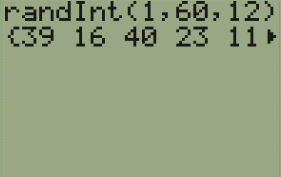
\includegraphics[width=1.6in]{samplingExRandInt3}
\end{center}
We start by looking for the 39th value in the list, then the 16th, and so on (this quickly gets tedious).  The result is
\[\boxed{7, 9, 9, 8, 7, 9, 10, 9, 8, 10, 8, 9}\]
and the average is
\begin{align*}
\textrm{Average score: } &= \dfrac{7+9+9+8+7+9+10+9+8+10+8+9}{12}\\
&= \boxed{8.6}
\end{align*}

\item To create a systematic sample, we simply need a starting point and a step size.  If we decide to pick every 3rd value, we can use the calculator to pick the starting point:
\begin{center}
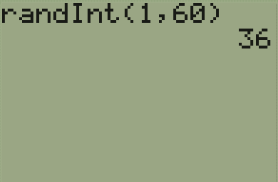
\includegraphics[width=1.6in]{samplingExRandInt4}
\end{center}
Starting at the 36th position and counting that value and every 3rd one after that yields the following sample:
\[\boxed{10, 7, 7, 7, 8, 3, 9, 8, 7, 9, 9, 9}\]
Notice that we wrapped around at the end of the list and came back to the beginning.  The average is
\begin{align*}
\textrm{Average score: } &= \dfrac{10+7+7+7+8+3+9+8+7+9+9+9}{12}\\
&= \boxed{7.8}
\end{align*}

\item Finally, a convenience sample simply means picking the easiest values; let's use the top two rows, since we can easily read and copy those without jumping around the table:
\[\boxed{5, 7, 10, 9, 8, 3, 10, 5, 9, 8, 7, 6}\]
\begin{align*}
\textrm{Average score: } &= \dfrac{5+7+10+9+8+3+10+5+9+8+7+6}{12}\\
&= \boxed{7.3}
\end{align*}
\end{enumerate}
\end{example}

Notice how the average for each sample was slightly different, but all relatively close to each other, ranging from 7.1 to 8.6.  This illustrates an important point: \textbf{different samples from the same population will give different results}, but as long as the sample size is not too small and the sample is not skewed or biased in some way, the results should be relatively similar.

Larger samples tend to be more consistent, but as we saw with the example of the \emph{Literary Digest}, larger sample sizes alone don't guarantee better outcomes.\\

This point about the natural variability of samples is a good one to keep in mind during election season, for instance, when multiple polls are released, and they all give different levels of support for one candidate or another.  A good approach is to compare a variety of reputable polls in order to gain a fuller picture; the website FiveThirtyEight, among others, does this well.